\documentclass[a4paper,12pt]{article}
\usepackage[margin=18mm]{geometry}
\usepackage{tikz}
\usepackage{amsmath}
\newcommand{\pFourCell}[2]{\makebox[#1em][c]{\ensuremath{#2}}}
\pagestyle{empty}
\begin{document}
\section*{Spaltentreue LaTeX-Ausgabe}
\noindent Gleichung: \texttt{sin(sqrt((x+3)/(2+1)))=5} \hfill Zielvariable: \texttt{x} \hfill Profil: \texttt{standard}

\vspace{8mm}
\begin{center}
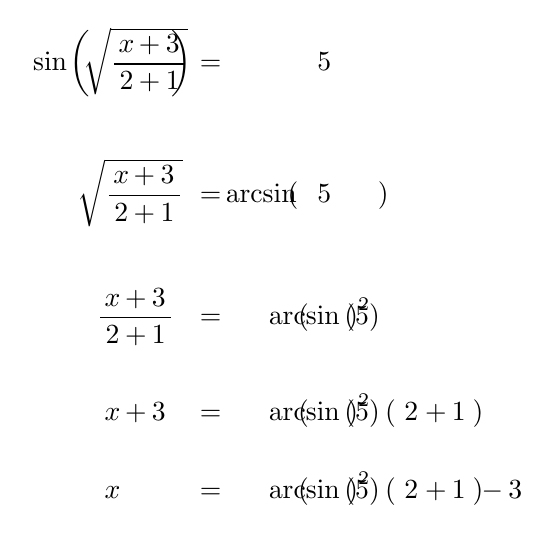
\begin{tikzpicture}[x=1em,y=-1em]
\node[anchor=base, inner sep=0pt] at (3.9,2.9) {$\pFourCell{2.56}{\sqrt{\displaystyle\frac{\pFourCell{0.9}{x}\pFourCell{0.78}{+}\pFourCell{0.88}{3}}{\pFourCell{0.9}{2}\pFourCell{0.78}{+}\pFourCell{0.88}{1}}}}$};
\node[anchor=base, inner sep=0pt] at (0.81,2.9) {$\pFourCell{1.62}{\sin}$};
\node[anchor=base, inner sep=0pt] at (1.93,2.9) {$\pFourCell{0.62}{\left(\vphantom{\pFourCell{2.56}{\sqrt{\displaystyle\frac{\pFourCell{0.9}{x}\pFourCell{0.78}{+}\pFourCell{0.88}{3}}{\pFourCell{0.9}{2}\pFourCell{0.78}{+}\pFourCell{0.88}{1}}}}}\right.}$};
\node[anchor=base, inner sep=0pt] at (5.49,2.9) {$\pFourCell{0.62}{\left.\vphantom{\pFourCell{2.56}{\sqrt{\displaystyle\frac{\pFourCell{0.9}{x}\pFourCell{0.78}{+}\pFourCell{0.88}{3}}{\pFourCell{0.9}{2}\pFourCell{0.78}{+}\pFourCell{0.88}{1}}}}}\right)}$};
\node[anchor=base, inner sep=0pt] at (6.61,2.9) {$=$};
\node[anchor=base, inner sep=0pt] at (10.72,2.9) {$5$};
\node[anchor=base, inner sep=0pt] at (3.71,7.65) {$\pFourCell{2.94}{\sqrt{\displaystyle\frac{\pFourCell{0.9}{x}\pFourCell{0.78}{+}\pFourCell{0.88}{3}}{\pFourCell{0.9}{2}\pFourCell{0.78}{+}\pFourCell{0.88}{1}}}}$};
\node[anchor=base, inner sep=0pt] at (6.61,7.65) {$=$};
\node[anchor=base, inner sep=0pt] at (10.72,7.65) {$\pFourCell{1}{5}$};
\node[anchor=base, inner sep=0pt] at (8.44,7.65) {$\pFourCell{2.04}{\arcsin}$};
\node[anchor=base, inner sep=0pt] at (9.65,7.65) {$\pFourCell{0.38}{\left(\vphantom{\pFourCell{1}{5}}\right.}$};
\node[anchor=base, inner sep=0pt] at (12.79,7.65) {$\pFourCell{0.38}{\left.\vphantom{\pFourCell{1}{5}}\right)}$};
\node[anchor=base, inner sep=0pt] at (3.9,12.075) {$\displaystyle\frac{\pFourCell{0.9}{x}\pFourCell{0.78}{+}\pFourCell{0.88}{3}}{\pFourCell{0.9}{2}\pFourCell{0.78}{+}\pFourCell{0.88}{1}}$};
\node[anchor=base, inner sep=0pt] at (6.61,12.075) {$=$};
\node[anchor=base, inner sep=0pt] at (10.72,12.075) {$\pFourCell{1}{\arcsin\left(5\right)}$};
\node[anchor=base, inner sep=0pt] at (10.03,12.075) {$\pFourCell{0.38}{\left(\vphantom{\pFourCell{1}{\arcsin\left(5\right)}}\right.}$};
\node[anchor=base, inner sep=0pt] at (11.91,12.075) {$\pFourCell{1.38}{\left.\vphantom{\pFourCell{1}{\arcsin\left(5\right)}}\right)^{2}}$};
\node[anchor=base, inner sep=0pt] at (3.07,15.535) {$x$};
\node[anchor=base, inner sep=0pt] at (3.91,15.535) {$+$};
\node[anchor=base, inner sep=0pt] at (4.74,15.535) {$3$};
\node[anchor=base, inner sep=0pt] at (6.61,15.535) {$=$};
\node[anchor=base, inner sep=0pt] at (10.72,15.535) {$\pFourCell{1}{\arcsin\left(5\right)}$};
\node[anchor=base, inner sep=0pt] at (10.03,15.535) {$\pFourCell{0.38}{\left(\vphantom{\pFourCell{1}{\arcsin\left(5\right)}}\right.}$};
\node[anchor=base, inner sep=0pt] at (11.91,15.535) {$\pFourCell{1.38}{\left.\vphantom{\pFourCell{1}{\arcsin\left(5\right)}}\right)^{2}}$};
\node[anchor=base, inner sep=0pt] at (14.69,15.535) {$\pFourCell{1}{2}\pFourCell{0.78}{+}\pFourCell{0.88}{1}$};
\node[anchor=base, inner sep=0pt] at (13.17,15.535) {$\pFourCell{0.38}{\left(\vphantom{\pFourCell{1}{2}\pFourCell{0.78}{+}\pFourCell{0.88}{1}}\right.}$};
\node[anchor=base, inner sep=0pt] at (16.21,15.535) {$\pFourCell{0.38}{\left.\vphantom{\pFourCell{1}{2}\pFourCell{0.78}{+}\pFourCell{0.88}{1}}\right)}$};
\node[anchor=base, inner sep=0pt] at (3.07,18.355) {$x$};
\node[anchor=base, inner sep=0pt] at (6.61,18.355) {$=$};
\node[anchor=base, inner sep=0pt] at (10.72,18.355) {$\pFourCell{1}{\arcsin\left(5\right)}$};
\node[anchor=base, inner sep=0pt] at (10.03,18.355) {$\pFourCell{0.38}{\left(\vphantom{\pFourCell{1}{\arcsin\left(5\right)}}\right.}$};
\node[anchor=base, inner sep=0pt] at (11.91,18.355) {$\pFourCell{1.38}{\left.\vphantom{\pFourCell{1}{\arcsin\left(5\right)}}\right)^{2}}$};
\node[anchor=base, inner sep=0pt] at (14.69,18.355) {$\pFourCell{1}{2}\pFourCell{0.78}{+}\pFourCell{0.88}{1}$};
\node[anchor=base, inner sep=0pt] at (13.17,18.355) {$\pFourCell{0.38}{\left(\vphantom{\pFourCell{1}{2}\pFourCell{0.78}{+}\pFourCell{0.88}{1}}\right.}$};
\node[anchor=base, inner sep=0pt] at (16.21,18.355) {$\pFourCell{0.38}{\left.\vphantom{\pFourCell{1}{2}\pFourCell{0.78}{+}\pFourCell{0.88}{1}}\right)}$};
\node[anchor=base, inner sep=0pt] at (16.79,18.355) {$-$};
\node[anchor=base, inner sep=0pt] at (17.62,18.355) {$3$};
\end{tikzpicture}
\end{center}

\newpage
\section*{Spaltentreue LaTeX-Ausgabe mit Spaltengrenzen}
\vspace{6mm}
\begin{center}
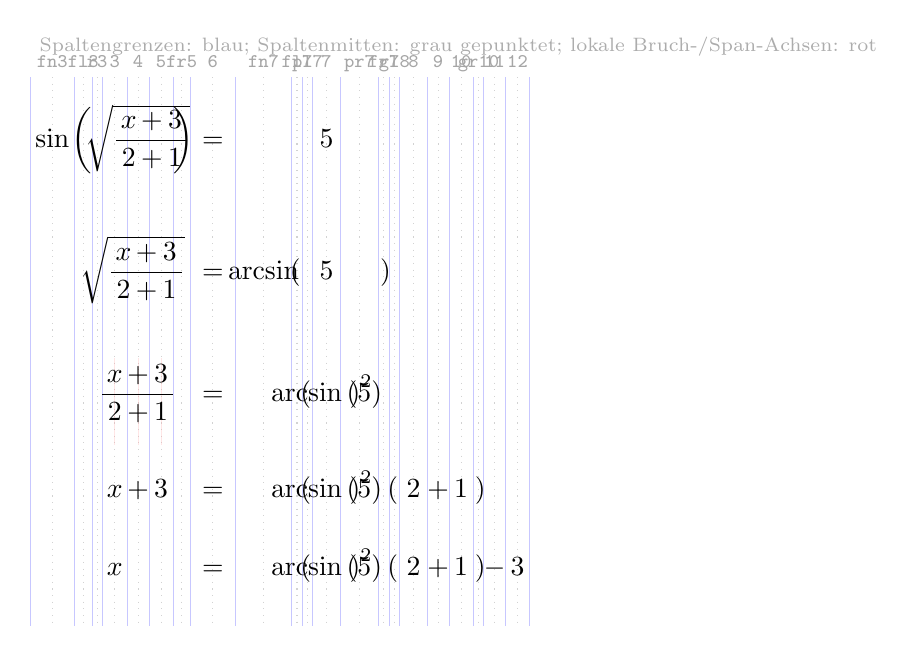
\begin{tikzpicture}[x=1em,y=-1em]
\node[font={\scriptsize}, text=gray!65, anchor=west] at (0,-0.75) {Spaltengrenzen: blau; Spaltenmitten: grau gepunktet; lokale Bruch-/Span-Achsen: rot};
\draw[blue!22, line width=0.28pt] (0,0.35) -- (0,20.19);
\draw[blue!22, line width=0.28pt] (1.62,0.35) -- (1.62,20.19);
\draw[blue!22, line width=0.28pt] (2.24,0.35) -- (2.24,20.19);
\draw[blue!22, line width=0.28pt] (2.62,0.35) -- (2.62,20.19);
\draw[blue!22, line width=0.28pt] (3.52,0.35) -- (3.52,20.19);
\draw[blue!22, line width=0.28pt] (4.3,0.35) -- (4.3,20.19);
\draw[blue!22, line width=0.28pt] (5.18,0.35) -- (5.18,20.19);
\draw[blue!22, line width=0.28pt] (5.8,0.35) -- (5.8,20.19);
\draw[blue!22, line width=0.28pt] (7.42,0.35) -- (7.42,20.19);
\draw[blue!22, line width=0.28pt] (9.46,0.35) -- (9.46,20.19);
\draw[blue!22, line width=0.28pt] (9.84,0.35) -- (9.84,20.19);
\draw[blue!22, line width=0.28pt] (10.22,0.35) -- (10.22,20.19);
\draw[blue!22, line width=0.28pt] (11.22,0.35) -- (11.22,20.19);
\draw[blue!22, line width=0.28pt] (12.6,0.35) -- (12.6,20.19);
\draw[blue!22, line width=0.28pt] (12.98,0.35) -- (12.98,20.19);
\draw[blue!22, line width=0.28pt] (13.36,0.35) -- (13.36,20.19);
\draw[blue!22, line width=0.28pt] (14.36,0.35) -- (14.36,20.19);
\draw[blue!22, line width=0.28pt] (15.14,0.35) -- (15.14,20.19);
\draw[blue!22, line width=0.28pt] (16.02,0.35) -- (16.02,20.19);
\draw[blue!22, line width=0.28pt] (16.4,0.35) -- (16.4,20.19);
\draw[blue!22, line width=0.28pt] (17.18,0.35) -- (17.18,20.19);
\draw[blue!22, line width=0.28pt] (18.06,0.35) -- (18.06,20.19);
\draw[gray!35, dotted] (0.81,0.35) -- (0.81,20.19);
\node[font={\ttfamily\scriptsize}, text=gray!70, anchor=base] at (0.81,0) {fn3};
\draw[gray!35, dotted] (1.93,0.35) -- (1.93,20.19);
\node[font={\ttfamily\scriptsize}, text=gray!70, anchor=base] at (1.93,0) {fl3};
\draw[gray!35, dotted] (2.43,0.35) -- (2.43,20.19);
\node[font={\ttfamily\scriptsize}, text=gray!70, anchor=base] at (2.43,0) {r3};
\draw[gray!35, dotted] (3.07,0.35) -- (3.07,20.19);
\node[font={\ttfamily\scriptsize}, text=gray!70, anchor=base] at (3.07,0) {3};
\draw[gray!35, dotted] (3.91,0.35) -- (3.91,20.19);
\node[font={\ttfamily\scriptsize}, text=gray!70, anchor=base] at (3.91,0) {4};
\draw[gray!35, dotted] (4.74,0.35) -- (4.74,20.19);
\node[font={\ttfamily\scriptsize}, text=gray!70, anchor=base] at (4.74,0) {5};
\draw[gray!35, dotted] (5.49,0.35) -- (5.49,20.19);
\node[font={\ttfamily\scriptsize}, text=gray!70, anchor=base] at (5.49,0) {fr5};
\draw[gray!35, dotted] (6.61,0.35) -- (6.61,20.19);
\node[font={\ttfamily\scriptsize}, text=gray!70, anchor=base] at (6.61,0) {6};
\draw[gray!35, dotted] (8.44,0.35) -- (8.44,20.19);
\node[font={\ttfamily\scriptsize}, text=gray!70, anchor=base] at (8.44,0) {fn7};
\draw[gray!35, dotted] (9.65,0.35) -- (9.65,20.19);
\node[font={\ttfamily\scriptsize}, text=gray!70, anchor=base] at (9.65,0) {fl7};
\draw[gray!35, dotted] (10.03,0.35) -- (10.03,20.19);
\node[font={\ttfamily\scriptsize}, text=gray!70, anchor=base] at (10.03,0) {pl7};
\draw[gray!35, dotted] (10.72,0.35) -- (10.72,20.19);
\node[font={\ttfamily\scriptsize}, text=gray!70, anchor=base] at (10.72,0) {7};
\draw[gray!35, dotted] (11.91,0.35) -- (11.91,20.19);
\node[font={\ttfamily\scriptsize}, text=gray!70, anchor=base] at (11.91,0) {pr7};
\draw[gray!35, dotted] (12.79,0.35) -- (12.79,20.19);
\node[font={\ttfamily\scriptsize}, text=gray!70, anchor=base] at (12.79,0) {fr7};
\draw[gray!35, dotted] (13.17,0.35) -- (13.17,20.19);
\node[font={\ttfamily\scriptsize}, text=gray!70, anchor=base] at (13.17,0) {gl8};
\draw[gray!35, dotted] (13.86,0.35) -- (13.86,20.19);
\node[font={\ttfamily\scriptsize}, text=gray!70, anchor=base] at (13.86,0) {8};
\draw[gray!35, dotted] (14.75,0.35) -- (14.75,20.19);
\node[font={\ttfamily\scriptsize}, text=gray!70, anchor=base] at (14.75,0) {9};
\draw[gray!35, dotted] (15.58,0.35) -- (15.58,20.19);
\node[font={\ttfamily\scriptsize}, text=gray!70, anchor=base] at (15.58,0) {10};
\draw[gray!35, dotted] (16.21,0.35) -- (16.21,20.19);
\node[font={\ttfamily\scriptsize}, text=gray!70, anchor=base] at (16.21,0) {gr10};
\draw[gray!35, dotted] (16.79,0.35) -- (16.79,20.19);
\node[font={\ttfamily\scriptsize}, text=gray!70, anchor=base] at (16.79,0) {11};
\draw[gray!35, dotted] (17.62,0.35) -- (17.62,20.19);
\node[font={\ttfamily\scriptsize}, text=gray!70, anchor=base] at (17.62,0) {12};
\node[anchor=base, inner sep=0pt] at (3.9,2.9) {$\pFourCell{2.56}{\sqrt{\displaystyle\frac{\pFourCell{0.9}{x}\pFourCell{0.78}{+}\pFourCell{0.88}{3}}{\pFourCell{0.9}{2}\pFourCell{0.78}{+}\pFourCell{0.88}{1}}}}$};
\node[anchor=base, inner sep=0pt] at (0.81,2.9) {$\pFourCell{1.62}{\sin}$};
\node[anchor=base, inner sep=0pt] at (1.93,2.9) {$\pFourCell{0.62}{\left(\vphantom{\pFourCell{2.56}{\sqrt{\displaystyle\frac{\pFourCell{0.9}{x}\pFourCell{0.78}{+}\pFourCell{0.88}{3}}{\pFourCell{0.9}{2}\pFourCell{0.78}{+}\pFourCell{0.88}{1}}}}}\right.}$};
\node[anchor=base, inner sep=0pt] at (5.49,2.9) {$\pFourCell{0.62}{\left.\vphantom{\pFourCell{2.56}{\sqrt{\displaystyle\frac{\pFourCell{0.9}{x}\pFourCell{0.78}{+}\pFourCell{0.88}{3}}{\pFourCell{0.9}{2}\pFourCell{0.78}{+}\pFourCell{0.88}{1}}}}}\right)}$};
\node[anchor=base, inner sep=0pt] at (6.61,2.9) {$=$};
\node[anchor=base, inner sep=0pt] at (10.72,2.9) {$5$};
\node[anchor=base, inner sep=0pt] at (3.71,7.65) {$\pFourCell{2.94}{\sqrt{\displaystyle\frac{\pFourCell{0.9}{x}\pFourCell{0.78}{+}\pFourCell{0.88}{3}}{\pFourCell{0.9}{2}\pFourCell{0.78}{+}\pFourCell{0.88}{1}}}}$};
\node[anchor=base, inner sep=0pt] at (6.61,7.65) {$=$};
\node[anchor=base, inner sep=0pt] at (10.72,7.65) {$\pFourCell{1}{5}$};
\node[anchor=base, inner sep=0pt] at (8.44,7.65) {$\pFourCell{2.04}{\arcsin}$};
\node[anchor=base, inner sep=0pt] at (9.65,7.65) {$\pFourCell{0.38}{\left(\vphantom{\pFourCell{1}{5}}\right.}$};
\node[anchor=base, inner sep=0pt] at (12.79,7.65) {$\pFourCell{0.38}{\left.\vphantom{\pFourCell{1}{5}}\right)}$};
\draw[red!30, opacity=0.32, line width=0.35pt] (3.07,10.5) -- (3.07,13.65);
\draw[red!30, opacity=0.32, line width=0.35pt] (3.91,10.5) -- (3.91,13.65);
\draw[red!30, opacity=0.32, line width=0.35pt] (4.74,10.5) -- (4.74,13.65);
\node[anchor=base, inner sep=0pt] at (3.9,12.075) {$\displaystyle\frac{\pFourCell{0.9}{x}\pFourCell{0.78}{+}\pFourCell{0.88}{3}}{\pFourCell{0.9}{2}\pFourCell{0.78}{+}\pFourCell{0.88}{1}}$};
\node[anchor=base, inner sep=0pt] at (6.61,12.075) {$=$};
\node[anchor=base, inner sep=0pt] at (10.72,12.075) {$\pFourCell{1}{\arcsin\left(5\right)}$};
\node[anchor=base, inner sep=0pt] at (10.03,12.075) {$\pFourCell{0.38}{\left(\vphantom{\pFourCell{1}{\arcsin\left(5\right)}}\right.}$};
\node[anchor=base, inner sep=0pt] at (11.91,12.075) {$\pFourCell{1.38}{\left.\vphantom{\pFourCell{1}{\arcsin\left(5\right)}}\right)^{2}}$};
\node[anchor=base, inner sep=0pt] at (3.07,15.535) {$x$};
\node[anchor=base, inner sep=0pt] at (3.91,15.535) {$+$};
\node[anchor=base, inner sep=0pt] at (4.74,15.535) {$3$};
\node[anchor=base, inner sep=0pt] at (6.61,15.535) {$=$};
\node[anchor=base, inner sep=0pt] at (10.72,15.535) {$\pFourCell{1}{\arcsin\left(5\right)}$};
\node[anchor=base, inner sep=0pt] at (10.03,15.535) {$\pFourCell{0.38}{\left(\vphantom{\pFourCell{1}{\arcsin\left(5\right)}}\right.}$};
\node[anchor=base, inner sep=0pt] at (11.91,15.535) {$\pFourCell{1.38}{\left.\vphantom{\pFourCell{1}{\arcsin\left(5\right)}}\right)^{2}}$};
\node[anchor=base, inner sep=0pt] at (14.69,15.535) {$\pFourCell{1}{2}\pFourCell{0.78}{+}\pFourCell{0.88}{1}$};
\node[anchor=base, inner sep=0pt] at (13.17,15.535) {$\pFourCell{0.38}{\left(\vphantom{\pFourCell{1}{2}\pFourCell{0.78}{+}\pFourCell{0.88}{1}}\right.}$};
\node[anchor=base, inner sep=0pt] at (16.21,15.535) {$\pFourCell{0.38}{\left.\vphantom{\pFourCell{1}{2}\pFourCell{0.78}{+}\pFourCell{0.88}{1}}\right)}$};
\node[anchor=base, inner sep=0pt] at (3.07,18.355) {$x$};
\node[anchor=base, inner sep=0pt] at (6.61,18.355) {$=$};
\node[anchor=base, inner sep=0pt] at (10.72,18.355) {$\pFourCell{1}{\arcsin\left(5\right)}$};
\node[anchor=base, inner sep=0pt] at (10.03,18.355) {$\pFourCell{0.38}{\left(\vphantom{\pFourCell{1}{\arcsin\left(5\right)}}\right.}$};
\node[anchor=base, inner sep=0pt] at (11.91,18.355) {$\pFourCell{1.38}{\left.\vphantom{\pFourCell{1}{\arcsin\left(5\right)}}\right)^{2}}$};
\node[anchor=base, inner sep=0pt] at (14.69,18.355) {$\pFourCell{1}{2}\pFourCell{0.78}{+}\pFourCell{0.88}{1}$};
\node[anchor=base, inner sep=0pt] at (13.17,18.355) {$\pFourCell{0.38}{\left(\vphantom{\pFourCell{1}{2}\pFourCell{0.78}{+}\pFourCell{0.88}{1}}\right.}$};
\node[anchor=base, inner sep=0pt] at (16.21,18.355) {$\pFourCell{0.38}{\left.\vphantom{\pFourCell{1}{2}\pFourCell{0.78}{+}\pFourCell{0.88}{1}}\right)}$};
\node[anchor=base, inner sep=0pt] at (16.79,18.355) {$-$};
\node[anchor=base, inner sep=0pt] at (17.62,18.355) {$3$};
\end{tikzpicture}
\end{center}
\end{document}
